\chapter{Introduction}

\section{General }
Universal language is a tool for machine thinking. It can not only execute code, but also infer rules. These processes are equivalent. Rules and inferences are the foundation of machine thinking. Firstly, they can define concepts, and secondly, they can explain principles of universal language and mathematics. 

Universal language structure: \\
data structure \(\rightarrow\) operations \(\rightarrow\) language system \(\rightarrow\) logic system \(\rightarrow\) propositions system \(\rightarrow\) axioms system \(\rightarrow\) theorems system.

Theorems system structure: \\
basic theorems system \(\rightarrow\) mathematics system \(\rightarrow\) virtual world system \(\rightarrow\) physical world system \(\rightarrow\) society.


\bigskip
\bigskip
\section{Data structure}
Universal language is based on data structure. The basic element of data structure is node. This data structure is tree-like multidimensional structure, and it is doubly linked circular in one dimension.   


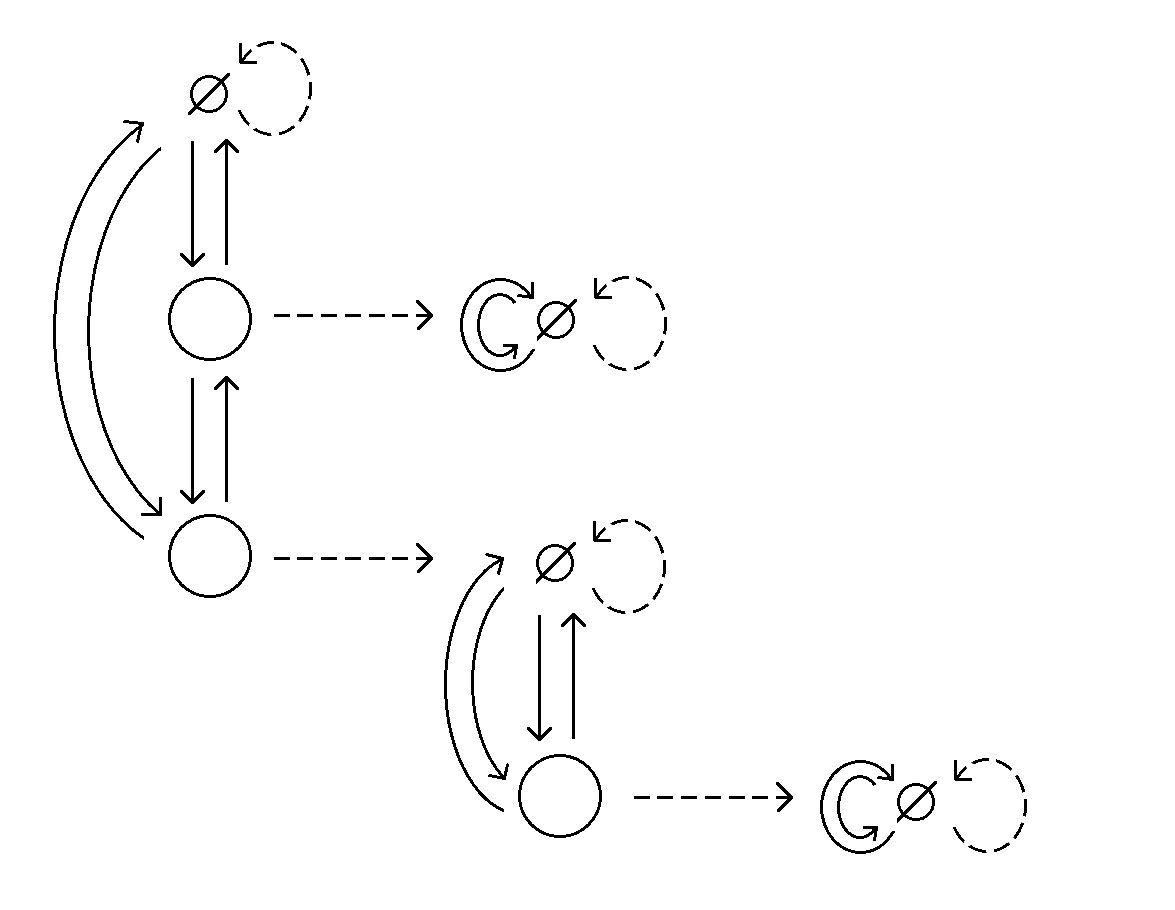
\includegraphics[scale = 0.5]{UL_datastrcuture.png}
\[Data  \; structure\]


\subsection{Node}
A node consists of:\\
1.	Data value.\\
2.	Link, pointing to the next node.\\
3.	Link, pointing to the previous node.\\
4.	Link, pointing to the child node.\\
5.	Unique node id.

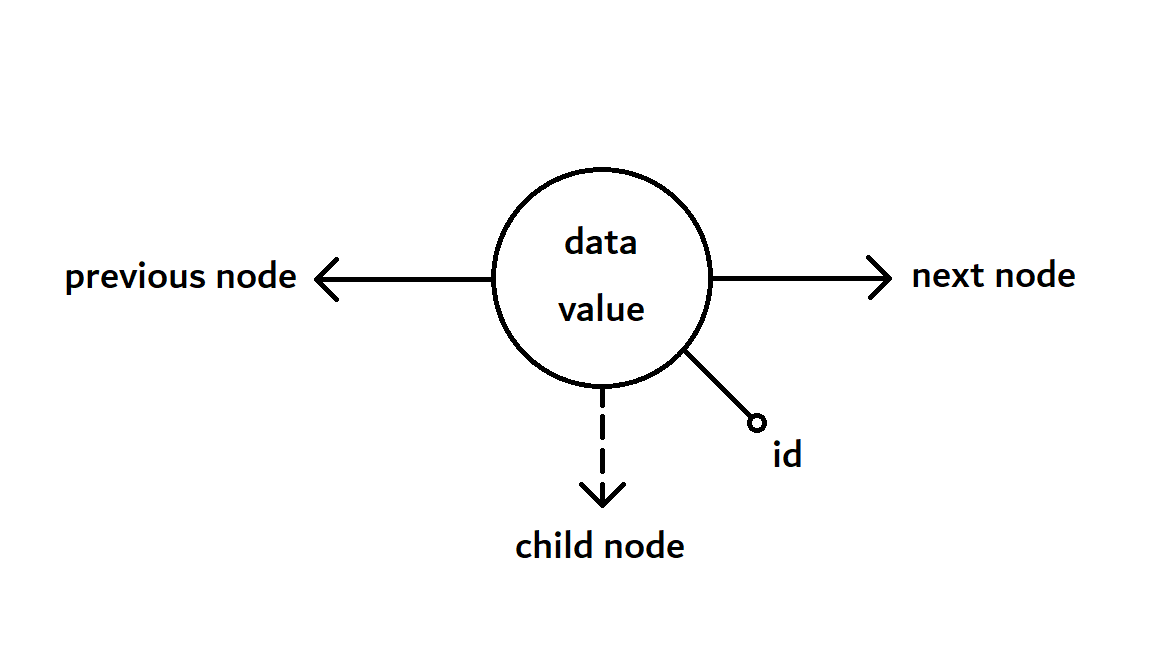
\includegraphics[scale = 0.5]{UL_node.png}
\[Node\]




\subsection{Empty node}
The empty node is \(\phi\). There is exactly one empty node in one dimension. An empty node is used to identify the start and end of a one-dimensional loop. An empty node has no child node, so it points to itself.



\bigskip
\bigskip
\section{Operations}
Operator is a Operation instruction. There are 11 operators:\\
\( \Og, \Ot, \Od, \Oc, \Ob, \Oe, \Oa, \On, \Op, \Os, \Or.\)


Operand is a variable expressed in conjunction with operators. An operand can be interpreted as a pointer to a node within a data structure.


An operation consists of an operator and several operands. Example:\\
\(i \Oc j\) is an operation, i and j is an operand, \(\Oc\) is an operator.\\\\ 
Operations:\\
\(\Og i \) : Create a new operand i, pointing to a unique global data structure.\\\\
\(\Ot i \) : Create a new operand i, pointing to a temporary newly allocated data structure.\\\\
\(i \Oc j \) : Create a new operand j. i and j point to the same node.\\\\
\(i \Od j \) : Create a new operand j pointing to a temporary newly allocated data structure. The data value of the node pointed to by j is the id of the node pointed to by i.\\\\
\(i \Ob j \) : Create a new operand j. j points to a child of the node pointed to by i.\\\\
\(i \Os \) : Release operand i. If i is the last operand that points to a temporary data structure, free the temporary data structure.\\\\
\(i \On \) : Move i to  the next node.\\\\
\(i \Op \) : Move i to  the previous node.\\\\
\(\Bb{i \Oe j}{,codeA,}{,codeB,} \) : Compare the value of the node pointed to by i with the value of the node pointed to by j. If equal, codeA executes, otherwise codeB executes.\\\\
\(i \Oa j \) : Insert a new non-empty node or delete a non-empty node.\\\\
\( \Or \) : Mean logic error and halt the program.\\\\
\includegraphics[scale = 0.5]{UL_node_op.png}
\[Node \; operation\]
\bigskip
\section{Language}
\subsection{Code}
	Code  consists of operations, functions, and “,”. “,” is  not only a connector for multiple operations but also   empty code. Code variables are represented as \(\Tc\) and alphanumerics, it represents anyone of the set of all code. \\
 The syntax of the code: \\
	Operand names cannot conflict. An existing operand cannot be created until it is released. A released operand can't be used  until it is created.


\subsection{Function}

Functions are how concepts are defined.

\subsubsection{Syntax of the function:}
“;” is the delimiter for operand parameters.

\( fn(L) \Rq codeA\). The input operands of codeA are the operands in the parameter list L, any operands created in codeA must be released in codeA.
  
\( fn(L):r \Rq codeB\). The input operands of codeB are the operands in the parameter list L, any operands created in codeB must be released in codeB except operand r. This is to ensure the closure of the function and to ensure consistency in the inference replacement process.

\subsubsection{The difference in functions:}

The name of the function: R(i), T(i) are different.
	

The number of parameters: Fn(i), Fn(i;j) are different.


The differences in parameter names:  Fn(i;j),Fn(j;i) are the same. Fn(i;j), Fn(i;i) are different. \( i \Pn j, i \Pn i\) are different.

\subsubsection{Type of functions:}
General function:
\[,Cpo(r), \Rq , r \Od m, m \Oa r, m \Os,\]

Branch function:
\[,\Blb{if(i \Pe j)}{,}{,} \Rq ,\Blb{i \Oe j}{,}{,}\]

Proposition function:
\[,i \Pe j, \Rq , \Bb{if(i \Pe j)}{,}{, \Or,}\]

Recursive function:
\[, R(i), \Rq , \Bb{if(i \Pu)}{,}{, i \On, R(i),}, \]

Return function:
\[, i +j:r, \Rq , \Ot r, i \Oc i_0, j \Oc j_0, r \Oc r_0, Rcpo(i_0;r_0), Rcpo(j_0;r_0), i_0 \Os, j_0 \Os, r_0 \Os, \]
r is return operand.



\subsection{Flag object}
Flag objects are named by “\&” and alphanumerics , and are used to represent special properties of data structures, operations, and codes. Flag objects are defined by rules. Flag objects can combine the symbol and operand parameters.Example:\\
\( \&SHi \Ps i, \; \&SHi \Pn i, \; \&Fam(i).\)



\bigskip
\bigskip
\section{Logic system}
\subsection{rule text}
A rule text consists of code, code variables, and flag objects. Rule text variables are named by \( \Tt\) and alphanumerics. It represents anyone of the set of all rule text.


\subsection{rule}
Given that A, B are rule text. The rule format : \(  A \Rq B\).

A rule is used to represent two equivalent rule text, which can replace each other. A, B must start and end with “,”.

When a code variable exists in a rule, it represents the set of all rules that replace the code variable with a code constant. Example:
\[\Brs{,}{,}, \Tc code, \Rq \Brs{, \Tc code, }{, \Tc code, }, \] 
means:
\[\Brs{,}{,}, \Or, \Rq \Brs{, \Or, }{, \Or, }, \] 

\[\Brs{,}{,}, \Ot i, i \Os, \Rq \Brs{, \Ot i, i \Os, }{, \Ot i, i \On, }, \] 

\[\Brs{,}{,}, i \On, \Rq \Brs{, i \On, }{, i \On, }, \] 
... ...

A rule has nothing to do with the naming of the operands in the rule, as long as the names do not conflict.
	Example:
\[,i \On, i \Op, \Rq , i \Op, i \On, \]
\[,j \On, j \Op, \Rq , j \Op, j \On, \]
the same rule.

\[, \Rq , \Ot i, i \Os, \]
\[, \Rq , \Ot j, j \Os, \]
the same rule.

\[,i \On, i \Op, \Rq , i \Op, i \On, \]
\[,i \On, j \Op, \Rq , j \Op, i \On, \]
different rules.

We simplify rule (\(  A \Rq A,B \) ) to rule(\(  A \Rq \sim,B \) ).

\subsection{inference}
Inference format: premise \( \Ri \) conclusion.

Inference: if the premise exists, then the conclusion exists. Inference can be axiom or theorem.

Premise can be one of more rules or inferences. Conclusion is a rule.

When there is a rule text variable in an inference, it represents the set of all inferences that replace the rule text variable with the rule text constant.

How to infer?

If inference (premise \( \Ri \) conclusion) exists and premise exists, then conclusion exists.

How to get an inference?

If the premise is assumed to exist, conclusion can be inferred. Then we can get an inference ( premise \( \Ri \) conclusion). If conclusion exists, then inference (any premise \( \Ri \) conclusion) always exists.





\subsection{Type of rule or inference}
\subsubsection{Axiom}
Axioms describe the natural properties of data structure, operations, code, and rule. Axioms do not need to be proved.

\subsubsection{Definition}
Concepts are defined by means of rules. A function is a definition. Flag objects can be defined by commutative rules.

\subsubsection{Theorem}
A theorem is a conclusion  of inference. A theorem  requires proof. 

\subsection{inference axiom of rule equivalence}
Given that A, B, M, N are rule text.

Equivalent commutativity:
\[ A \Rq B \Ri B \Rq A\]

Equivalent transitivity:
\[\Bigl\{ ^{A \Rq B}_{B \Rq C}\Bigl\} \Ri A \Rq C\]


Equivalent substitution:
\[ A \Rq B \Ri M A N \Rq M B N\]

Rule text(M A N) and rule text(M B N)  must not have naming conflicts. rule text A and rule text B must be in the same “,” start position and “,” end position.

naming conflict:
\[, \Rq , i \Oc j, j \Os, \Ri , j \On, \Rq , j \On, i \Oc j, j \Os,\]
should be:
\[, \Rq , i \Oc t, t \Os, \Ri , j \On, \Rq , j \On, i \Oc t, t \Os,\]

naming conflict:
\[, \Ot i,  \Rq , \Ot i, i \nPs j, \Ri , j \Os, \Ot i, \Rq , j \Os, \Ot i, i \nPs j, \]
should be:
\[, \Ot i,  \Rq , \Ot i, i \nPs t, \Ri , j \Os, \Ot i, \Rq , j \Os, \Ot i, i \nPs t,\]

\subsection{contradiction rule}
Contradiction rule:
\[, \Rq , \Or, \]

If inference(premise \( \Ri , \Rq , \Or, \)) exists, then premise is not compatible with existing system. Premise can be axiom or definition. The contradiction rule is not compatible with existing system. 


\subsection{proof}
Example:
\[,i \On, j \Op, \Rq , j \Op, i \On,\]
proof:\\
\begin{math}
inference:Equivalent \, substitution.\\
premise: \; , \Rq , j \On, j \Op,(axiom)\\
conclusion: \; ,i \On, j \Op,\Rq, j \On, j \Op, i \On, j \Op,\\
\\
inference:Equivalent \, substitution.\\
premise:  \; , j \On, j \Op, \Rq , j \Op, j \On,(axiom)\\
conclusion: \; , j \On, j \Op, i \On, j \Op, \Rq , j \Op, j \On, i \On, j \Op,\\
\\
inference:Equivalent \, transitivity.\\
premise1: \; ,i \On, j \Op,\Rq, j \On, j \Op, i \On, j \Op,\\
premise2: \; , j \On, j \Op, i \On, j \Op, \Rq , j \Op, j \On, i \On, j \Op,\\
conclusion: \; , i \On, j \Op, \Rq , j \Op, j \On, i \On, j \Op,\\
\\
inference:Equivalent \, substitution.\\
premise: \;  , j \On, i \On, \Rq , i \On, j \On,(axiom)\\
conclusion: \; , j \Op, j \On, i \On, j \Op, \Rq , j \Op, i \On, j \On, j \Op,\\
\\
inference:Equivalent \, transitivity.\\
premise1: \; , i \On, j \Op, \Rq , j \Op, j \On, i \On, j \Op,\\
premise2: \; , j \Op, j \On, i \On, j \Op, \Rq , j \Op, i \On, j \On, j \Op,\\
conclusion: \; , i \On, j \Op, \Rq , j \Op, i \On, j \On, j \Op,\\
\\
inference:Equivalent \, commutativity.\\
premise: \;  , \Rq , j \On, j \Op,(axiom)\\
conclusion: \; , j \On, j \Op, \Rq ,\\
\\
inference:Equivalent \, substitution.\\
premise: \;  , j \On, j \Op, \Rq ,(proved)\\
conclusion: \; , j \Op, i \On, j \On, j \Op, \Rq , j \Op, i \On,\\
\\
inference:Equivalent \, transitivity.\\
premise1: \; , i \On, j \Op, \Rq , j \Op, i \On, j \On, j \Op,\\
premise2: \; , j \Op, i \On, j \On, j \Op, \Rq , j \Op, i \On,\\
conclusion: \; , i \On, j \Op, \Rq , j \Op, i \On,\\
\\
simplify:\\
,i \On, j \Op, \\\\
\Rq, j \On, j \Op, i \On, j \Op,( , \Rq , j \On, j \Op,) \\\\
\Rq, j \Op, j \On, i \On, j \Op, (, j \On, j \Op, \Rq , j \Op, j \On,)\\\\
\Rq, j \Op, i \On, j \On, j \Op, (, j \On, i \On, \Rq , i \On, j \On,)\\\\
\Rq, j \Op, i \On,( , \Rq , j \On, j \Op,)\\\\
Minimize:\\
,i \On, j \Op, \\\\
\Rq, j \On, j \Op, i \On, j \Op, \\\\
\Rq, j \Op, j \On, i \On, j \Op, \\\\
\Rq, j \Op, i \On, j \On, j \Op, \\\\
\Rq, j \Op, i \On,
\end{math}
\bigskip
\bigskip



\bigskip
\bigskip
\section{Propositions system}
We describe laws and properties through propositions. Propositions come from operator of equal comparison(\(\Bls{i \Oe j}{,}{,} \)), but only one branch can be executed depending on the axioms.

Before defining propositions , we should define branch function(\(\Bls{if(p)}{,}{,} \)).

Definition of propositions:
\[,p, \Rq ,\Bb{if(p)}{,}{, \Or, },\]

and

\[,!p, \Rq ,\Bb{if(p)}{, \Or,}{, },\]




\newpage